\section{Formal Syntax Rules}

\subsection{Formal Language}
A formal language \(L\) over an alphabet \(\Sigma\) is a subset of \(\Sigma^*\), which is the set of strings consisting of and making use of elements in \(\Sigma\). The empty string is denoted by \(\varepsilon\). 

For example, a formal language \(L\) over \(\Sigma = \{1, 2\}\) is a subset of \(\Sigma^*\), e.g. \(L = \{\varepsilon, 1, 2, 11, 22, 111, 222\}\). 

One way to manipulate strings is using a rewriting system, which consists of rules that map strings in a formal language to other strings in the language. For a language \(L\), we define a relation \(\to\) over strings in \(L\). For example, for \(L = \{1, 2, 11\}\), we may have \(\to = \{(1, 2), (2, 1), (1, 11), (11, 2)\}\). Then we can write \(1 \to 2\), \(2 \to 1\), \(1 \to 11\), and \(11 \to 2\). 

We also have generative grammar, which is a kind of rewriting system over a language \((\Sigma \cup N)^*\), where

- the alphabet is partitioned into two sets: a set of non-terminal symbols \(N\) and a set of terminal symbols \(\Sigma\),

- there is a distinguished start symbol in \(N\),

- rewrite rules are called \textit{production rules}; the left-hand side of each rule contains at least one non-terminal. 

We can use generative grammars to define a language over the alphabet \(\Sigma\). The language defined is the set of strings of terminal symbols that we can generate by starting with the start symbol \(S\) and following the production rules. 

\begin{eg}[Generative Grammar]
Consider \(\Sigma \equiv \{a, b, c\}\).

\textbf{Language ONE} with only two strings \(\{a, b\}\). 

In this case, to generate a language over \(\Sigma\), we have \(N = \{S\}, \Sigma = \{a, b, c\}\) with grammar (production rules): 
\[
\begin{aligned}
  S \to a \\
  S \to b
\end{aligned}
\]

\textbf{Language A-B} where no \(a\) follows any \(b\), e.g. \(\varepsilon, ab, aab, acb\). 

In this case, consider \(N = \{S, A, B, C\}, \Sigma = \{a, b, c\}\) with production rules: 
\[
\begin{aligned}
  S &\to CABC \\
  C &\to \varepsilon \quad C \to cC \\
  A &\to \varepsilon \quad A \to aCA \\
  B &\to \varepsilon \quad B \to bCB \\
\end{aligned}
\]

\textbf{Language MATCH} where the number of \(a\)s and \(b\)s is the same.  

In this case, consider \(N = \{S\}, \Sigma = \{a, b, c\}\) with production rules: 
\[
\begin{aligned}
  S &\to \varepsilon \quad\quad S \to c \\
  S &\to aSb \quad S \to bSa \\
  S &\to SS
\end{aligned}
\]

\begin{minipage}{0.49\textwidth}
\begin{figure}[H]
  \centering
  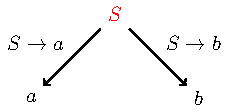
\includegraphics[width=0.5\textwidth]{Figure/1.1.1_1.pdf}
\end{figure}
\end{minipage}
\begin{minipage}{0.49\textwidth}
\begin{figure}[H]
  \centering
  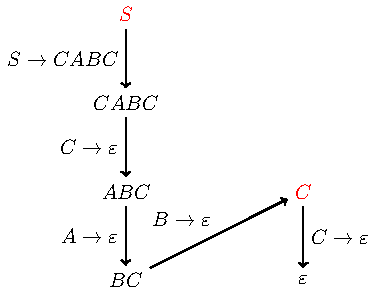
\includegraphics[width=0.7\textwidth]{Figure/1.1.1_2.pdf}
\end{figure}
\end{minipage}
\end{eg}

\subsection{Context-Free Grammar (CFGs)}
The above grammars are context-free grammars, where the left-hand side of each production rule consists of a single non-terminal. It is often specified using Backus-Naur Form (BNF), where

- every production rule is written with \(\Coloneqq\) instead of \(\to\),

- production rules with the same left-hand side are combined into a single rule, where different right-hand sides are separated with \(\vert\), e.g. Language BOOL of boolean formulas with 

- conjunction (and) \(\wedge\) 

- disjunction (or) \(\vee\) 

- negation (not) \(\neg\) 
\[
  S \Coloneqq x \mid y \mid z \mid w \mid (S) \mid S \wedge S \mid S \vee S \mid \neg S
\]

\begin{eg}[BNF]
  Consider a BNF grammar for \(\text{LUNCH}^-\).
  \[
  \begin{aligned}
    S &\Coloneqq NP\ VP. \\
    NP &\Coloneqq N \mid N\ PP \\
    VP &\Coloneqq V \mid V\ NP \mid V\ PP \mid V\ NP\ PP \\
    V &\Coloneqq \text{buys} \mid \text{eats}  \\
    N &\Coloneqq \text{Alice} \mid \text{Bob} \mid \text{soup} \mid \text{salad} \mid \text{pizza} \\
    PP &\Coloneqq \text{in a bowl} \mid \text{in a teacup} \mid \text{in a house} \\
  \end{aligned}
  \]
  \begin{minipage}{0.5\textwidth}    
  Then we can derive a derivation tree (parse tree):
  \[
  \begin{aligned}
    S &\to \textcolor{red}{NP}\ VP. \\
    &\to \textcolor{red}{N}\ VP. \\
    &\to \text{Alice } \textcolor{red}{VP}. \\
    &\to \text{Alice } \textcolor{red}{V}NP. \\
    &\to \text{Alice eats } \textcolor{red}{NP}. \\
    &\to \text{Alice eats } \textcolor{red}{N}. \\
    &\to \text{Alice eats soup.} \\
  \end{aligned}
  \]
  \end{minipage}
  \begin{minipage}{0.5\textwidth}    
  \begin{center}
  \begin{forest}
  for tree={
    math content,
    s sep=20pt,
    l sep=20pt
  }
  [S
    [NP [N [\text{Alice}]]]
    [VP
        [V [\text{eats}]]
        [NP [N [\text{soup}]]]
    ]
    [.]
  ]
  \end{forest}
  \end{center}
  \end{minipage}
\end{eg}

\begin{remark}
  A parse tree acts as a proof that a string is in a language (membership). 
\end{remark}

\subsection{Ambiguity \& \textit{Dangling Else Problem}}
A grammar is ambiguous if the same string has more than one parse tree, e.g.

\begin{minipage}{0.5\textwidth}
\begin{forest}
  for tree={
    math content,
    s sep=20pt,
    l sep=20pt
  }
  [S
    [NP [N [\text{Alice}]]]
    [VP
        [V [\text{eats}]]
        [NP
            [N [\text{noodles}]]
            [PP [\text{in a teacup}]]
        ]
    ]
    [.]
  ]
\end{forest}
\end{minipage}
\begin{minipage}{0.5\textwidth}
\begin{forest}
for tree={
  math content,
  s sep=20pt,
  l sep=20pt
}
[S
  [NP [N [\text{Alice}]]]
  [VP
      [V [\text{eats}]]
      [NP [N [\text{noodles}]]]
      [PP [\text{in a teacup}]]
      ]
  [.]
]
\end{forest}
\end{minipage}

Grammar serves an additional purpose, that is, it can be used to give structure to a string in a language. Semantics for the strings within a language are typically described with respect to this additional structure imposed on the string. Ambiguous grammar can thus lead to ambiguous meanings being assigned to strings. 

For example, in the above examples, the left suggests that the noodles are in a teacup, whereas the right one suggests that Alice is located in a teacup. While one interpretation may be more likely than another and judgment can be based on semantics and background knowledge, the correct conclusion is not determined by the grammar alone. 

This problem can manifest in the \textit{dangling else problem} in a programming language context. 

Consider language IF with the following grammar:
\[
\begin{aligned}
  S &\Coloneqq C \mid \text{ if } B \text{ then } S \mid \text{ if } B \text{ then } S \text{ else } S \\
  B &\Coloneqq \text{ true } \mid \text{ false } \mid \dots \\ 
  C &\Coloneqq \dots 
\end{aligned}
\]

To deal with ambiguity, we can

1. change the grammar such that it is \textbf{not} ambiguous, i.e. same language with a different grammar.

For example, for BOOL:
\[
  S \Coloneqq x \mid y \mid z \mid w \mid (S) \mid S \wedge S \mid S \vee S \mid \neg S
\]
we change to 
\[
\begin{aligned}
  S &\Coloneqq D \vee S \mid D \\
  D &\Coloneqq C \wedge D \mid C \\
  C &\Coloneqq (S) \mid \neg C \mid x \mid y \mid z \mid w \\
\end{aligned}
\]

2. change the syntax, i.e. a different language with a different grammar.

For example, we change language IF to 
\[
  S \Coloneqq C \mid \text{ if } B \text{ then } S \text{ end if } \mid \text{ if } B \text{ then } S \text{ else } S \text{ end if }
\]

\section{Abstract syntax trees (ASTs)}
Before, we have \(\mathsf{Interpreter}_{\mathcal{L}}\) for \(\mathcal{L}\) that takes a program in \(\mathcal{L}\) and produces a value. Typically, there is a frontend containing a \textit{parser} and a backend containing an \textit{evaluator}. The parser parses the input string according to a grammar and converts the input program into an intermediate representation called an abstract syntax tree (AST),
\[
  \textsf{Parser}_{\mathcal{L}}: \mathcal{L} \to \text{AST}(\mathcal{L}) 
\] 
and the evaluator then evaluates the AST to a value,
\[
  \textsf{Evaluator}_{\text{AST}(\mathcal{L})} : \text{AST}(\mathcal{L}) \to \mathcal{V}
\]
Then we have 
\[
  \textsf{Interpreter}_{\mathcal{L}} = \textsf{Evaluator}_{\text{AST}(\mathcal{L})} \circ \textsf{Parser}_{\mathcal{L}} 
\]

The AST representation abstracts a parse tree and keeps only the relevant syntactic information from the parse tree, in particular, a subset of the production rules applied to obtain the parse tree. 

To make an AST:

1. derive a parse tree annotated with (important) production rules applied,

2. remove terminal nodes,

3. remove nodes expanded by production rules we do not care about; on removal, parent the node's children to its parent,

4. relabel non-terminal nodes with the annotated production rule names.

For example, for \(x \wedge y \vee z\) with 
\[
\begin{aligned}
  S &\Coloneqq D \vee S \mid D \\
  D &\Coloneqq C \wedge D \mid C \\
  C &\Coloneqq (S) \mid \neg C \mid x \mid y \mid z \mid w \\
\end{aligned}
\]
we have

\begin{minipage}{0.4\textwidth} 
  \begin{forest} 
    for tree={ 
      math content, % Automatically wraps node text in $ $ 
      s  sep=20pt, % Horizontal spacing 
      l sep=20pt % Vertical spacing between levels 
    } 
    [S \text{ (OR)} 
      [D \text{ (AND)} 
        [C(x) [\textcolor{red}{x}]] 
        [\textcolor{red}{\wedge}] 
        [D 
          [C(y) [\textcolor{red}{y}]]
        ]
      ] 
      [\textcolor{red}{\vee}] 
      [S 
        [D 
          [C(z) [\textcolor{red}{z}]]
        ]
      ] 
    ] 
  \end{forest}
\end{minipage}
\begin{minipage}{0.3\textwidth}
  \begin{forest} 
    for tree={ 
      math content, % Automatically wraps node text in $ $ 
      s  sep=20pt, % Horizontal spacing 
      l sep=20pt % Vertical spacing between levels 
    } 
    [S \text{ (OR)} 
      [D \text{ (AND)} 
        [C(x)] 
        [\textcolor{red}{D} [C(y)]] 
      ] 
      [\textcolor{red}{S} 
        [\textcolor{red}{D} [C(z)]]
      ] 
    ] 
  \end{forest} 
\end{minipage} 
\begin{minipage}{0.3\textwidth} 
  \begin{forest} 
    for tree={ 
        math content, % Automatically wraps node text in $ $ 
        s  sep=20pt, % Horizontal spacing 
        l sep=20pt % Vertical spacing between levels 
    } 
    [S \text{ (OR)} 
      [D \text{ (AND)} 
        [C\ (x)] 
        [C\ (y)] 
      ] 
      [C\ (z)] ] 
  \end{forest} 
\end{minipage}

finally we have 
\begin{center}
\begin{forest}
  for tree={
    math content,
    s sep=20pt,
    l sep=20pt
  }
  [\text{OR}
    [\text{AND}
      [x]
      [y]
    ]
    [z]
  ]
\end{forest}
\end{center}

Notice that we have viewed ASTs as generic trees, but they are often trees with a specific structure, i.e. nodes with a certain label might always have a particular degree or children that have only certain kinds of labels. This structure can be captured by another grammar, where we introduce a production rule in the AST grammar for each production rule that we care about. For example, for the above BOOL, we might have the following grammar:
\[
  AST \Coloneqq OR(AST, AST) \mid AND(AST, AST) \mid NOT(AST) \mid x \mid y \mid z \mid w
\]

This can be directly translated into an ADT, such as the following in OCaml:

\begin{lstlisting}[language=OCaml]
type bool_ast = Or of bool_ast * bool_ast
  | And of bool_ast * bool_ast
  | Not of bool_ast
  | X
  | Y
  | Z
  | W
\end{lstlisting}

The \texttt{bool\_ast} for \(x \wedge y \vee z\) is \texttt{Or(And(X,Y),Z)}.

When implementing a parser, rather than generating a full parse tree and then an AST, we can generate the AST during parsing by applying the appropriate ADT constructor for a production rule. 

\section{Beyond BNF and Meta-variables}
Many programming languages use formal grammars to specify syntax, yet they do not directly use BNF. Instead, they use \textbf{extensions} or \textbf{variants} of BNF. 

For example, in the language BOOL, we have 
\[
  Vars \cup \{\wedge, \vee, \neg, (,)\}
\]
and in the grammar each variable in \(Vars\) becomes a terminal in the production rules. To extend BOOL such that it allows more variables requires updating the BNF grammar with new production rules. However, when we want to allow infinitely many variable names, this becomes impossible as BNF grammars are finite. 

We then use extensions of BNF which allow using additional notations outside of BNF, e.g. \textit{meta-variables}. For example, let \(BoolVars\) be an infinite set of variables and let \(v\) range over \(BoolVars\); then \(v\) is a stand-in for any element of \(BoolVars\). Then we can still construct parse trees using BNF-like grammars and derive ASTs for them as before. 

For example, consider the BNF grammar:
\[
\begin{aligned}
  S &\Coloneqq Z \mid Z + S \\
  Z &\Coloneqq -N \mid N \\
  N &\Coloneqq DN \mid D \\
  D &\Coloneqq 0 \mid 1 \mid 2 \mid 3 \mid 4 \mid 5 \mid 6 \mid 7 \mid 8 \mid 9
\end{aligned}
\]
We typically write this as:

For \(z\) ranging over integers: 
\[
  S \Coloneqq z \mid z + S
\]
Here \(z\) is an integer, which is a semantic constraint, and this form of grammar is technically an extension of BNF. 

For example, we have a parse tree and AST for \(1 + 2 + 3\) as: 

\begin{minipage}{0.5\textwidth}
\begin{center}
\begin{forest}
  for tree={
    math content,
    s sep=20pt,
    l sep=20pt
  }
  [S (S \to 1 + S)
    [1]
    [+]
    [S (S \to 2 + S)
      [2]
      [+]
      [S (S \to 3)
        [3]
      ]
    ]
  ]
\end{forest}
\end{center}
\end{minipage}
\begin{minipage}{0.5\textwidth}
\begin{center}
\begin{forest}
  for tree={
    math content,
    s sep=20pt,
    l sep=20pt
  }
  [1+
    [2+ 
      [3]
    ]
  ]
\end{forest}
\end{center}
\end{minipage}

However, consider tracking chosen \(z\) values, treating \(z\) as if generated by an infinite set of production rules:
\[
  z \in Z \Coloneqq \dots \mid -1 \mid 0 \mid 1 \mid \dots 
\]
Then we have 

\begin{minipage}{0.5\textwidth}
\begin{center}
\begin{forest}
  for tree={
    math content,
    s sep=20pt,
    l sep=20pt
  }
  [S (S \to z + S)
    [\text{choose } 1 [1]]
    [+]
    [S (S \to z + S)
      [\text{choose } 2 [2]]
      [+]
      [S (S \to z)
        [\text{choose } 3 [3]]
      ]
    ]
  ]
\end{forest}
\end{center}
\end{minipage}
\begin{minipage}{0.5\textwidth}
\begin{center}
\begin{forest}
  for tree={
    math content,
    s sep=20pt,
    l sep=20pt
  }
  [+
    [1]
    [+
      [2] 
      [3]
    ]
  ]
\end{forest}
\end{center}
\end{minipage}

Note that an AST is an abstraction of the original parse tree that retains semantically meaningful parts. Choices of meta-variables are usually important. 

For the above example, there is another grammar that generates the same language, i.e.
\[
  S^{\prime} \Coloneqq z \mid S^{\prime} + S^{\prime} 
\]
For example, we have

\begin{minipage}{0.5\textwidth}
\begin{center}
\begin{forest}
  for tree={
    math content,
    s sep=20pt,
    l sep=20pt
  }
  [S \textcolor{red}{(S \to z + S)}
    [\text{choose } 1 [1]]
    [+]
    [S \textcolor{red}{(S \to z + S)}
      [\text{choose } 2 [2]]
      [+]
      [S \textcolor{gray}{(S \to z)}
        [\text{choose } 3 [3]]
      ]
    ]
  ]
\end{forest}
\end{center}
\end{minipage}
\begin{minipage}{0.5\textwidth}
\begin{center}
\begin{forest}
  for tree={
    math content,
    s sep=20pt,
    l sep=20pt
  }
  [S^{\prime} \textcolor{red}{(S^{\prime} \to S^{\prime} + S^{\prime})}
    [S^{\prime} \textcolor{gray}{(S^{\prime} \to z)} [\text{choose } 1 [1]]]
    [+]
    [S^{\prime} \textcolor{red}{(S^{\prime} \to S^{\prime} + S^{\prime})}
      [S^{\prime} \textcolor{gray}{(S^{\prime} \to z)} [\text{choose } 2 [2]]]
      [+]
      [S^{\prime} \textcolor{gray}{(S^{\prime} \to z)} [\text{choose } 3 [3]]]
    ]
  ]
\end{forest}
\end{center}
\end{minipage}

which give the same AST. 

So consider \(S^{\prime} \Coloneqq z \mid S^{\prime} + S^{\prime}\). If \(+\) is left-associative, then the left-most \(+\) will bind most tightly. We then expect this \(+\) to be closest to the leaves in the AST, and the left operation is evaluated first.

\begin{minipage}{0.5\textwidth}
\begin{center}
\begin{forest}
  for tree={
    math content,
    s sep=20pt,
    l sep=20pt
  }
  [+
    [+ 
      [1]
      [2]
    ]
    [3]
  ]
\end{forest}
\captionof{figure}{Left Associative}
\end{center}
\end{minipage}
\begin{minipage}{0.5\textwidth}
\begin{center}
\begin{forest}
  for tree={
    math content,
    s sep=20pt,
    l sep=20pt
  }
  [+
    [1]
    [+
      [2] 
      [3]
    ]
  ]
\end{forest}
\captionof{figure}{Right Associative}
\end{center}
\end{minipage}

To further reduce ambiguity, we can add a meta-variable \(a\) that ranges over strings generated by the grammar \(S^{\prime} \Coloneqq z \mid S^{\prime} + S^{\prime}\), i.e.
\[
  a \in S^{\prime} \Coloneqq z \mid a_1 + a_2
\]
where \(+\) is right-associative (by declaring the type of associativity to reduce ambiguity). 

Then consider BOOL again. We can use meta-variables and BNF-like syntax to allow variable names to be anything in the possibly infinite set \(BoolVars\), e.g.
\[
  S \Coloneqq v \mid (S) \mid S \wedge S \mid S \vee S \mid \neg S
\]
and to remove ambiguity, we can specify the \textit{precedence} and \textit{associativity} of \(\wedge, \vee, \neg\). 

The OCaml ADT for the structure of the ASTs for \(\textsc{BOOL}^+\) could be something like 
\begin{lstlisting}[language=OCaml]
type bool_ext_ast = Or of bool_ext_ast * bool_ext_ast
  | And of bool_ext_ast * bool_ext_ast
  | Not of bool_ext_ast
  | Var of string
\end{lstlisting}